\begin{ccRefFunction}{compare_x}

\ccFunction{Comparison_result compare_x(const Point_2<Kernel> &p,
                                        const Point_2<Kernel> &q);}
        {compares the $x$-coordinates of $p$ and $q$.}

\ccFunction{Comparison_result compare_x(const Point_3<Kernel> &p,
                                        const Point_3<Kernel> &q);}
        {compares the $x$-coordinates of $p$ and $q$.}

\begin{ccTexOnly}
\begin{figure}[hb]
\centerline{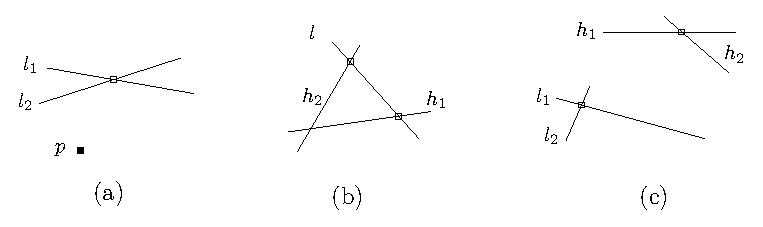
\includegraphics{Kernel_23_ref/fig/compare1}}
\caption{Comparison of the $x$ or $y$-coordinates of the (implicitly
given) points in the boxes.\label{fig-compare}}
\end{figure} 
\end{ccTexOnly} 

\ccFunction{Comparison_result compare_x(const Point_2<Kernel> &p,
                                        const Line_2<Kernel> &l1,
                                        const Line_2<Kernel> &l2);}
        {compares the $x$-coordinates of $p$ and the \ccHtmlNoLinksFrom{intersection} 
         of lines $l1$ and $l2$% 
         \ccTexHtml{ (Figure~\ref{fig-compare} (a))}{, see (a) in the figure 
         below}.}


\ccFunction{Comparison_result compare_x(const Line_2<Kernel> &l,
                                        const Line_2<Kernel> &h1,
                                        const Line_2<Kernel> &h2);}
        {compares the $x$-coordinates of  the \ccHtmlNoLinksFrom{intersection} of line $l$
         with line $h1$ and with line $h2$%
         \ccTexHtml{ (Figure~\ref{fig-compare} (b))}{, see (b) in the figure 
         below}.}


\ccFunction{Comparison_result compare_x(const Line_2<Kernel> &l1,
                                        const Line_2<Kernel> &l2,
                                        const Line_2<Kernel> &h1,
                                        const Line_2<Kernel> &h2);}
        {compares the $x$-coordinates of the \ccHtmlNoLinksFrom{intersection} of lines $l1$
         and $l2$ and  the \ccHtmlNoLinksFrom{intersection} of lines $h1$ and $h2$%
         \ccTexHtml{ (Figure~\ref{fig-compare} (c))}{, see (c) in the figure 
         below}.}

\begin{ccHtmlOnly}
<img border=0 src="fig/compare1.gif" align=center alt="Comparison of the x 
or y coordinates of the (implicitly given) points in the boxes">
\end{ccHtmlOnly} 

\ccSeeAlso
\ccRefIdfierPage{CGAL::compare_xy} \\
\ccRefIdfierPage{CGAL::compare_xyz} \\
\ccRefIdfierPage{CGAL::compare_x_at_y} \\
\ccRefIdfierPage{CGAL::compare_y} \\
\ccRefIdfierPage{CGAL::compare_yx} \\
\ccRefIdfierPage{CGAL::compare_y_at_x} \\
\ccRefIdfierPage{CGAL::compare_z} \\

\end{ccRefFunction}

